\section{Durchführung}
\label{sec:Durchführung}
Bei dem im Versuch verwendeten $\alpha$-Strahler handelt es sich um $\ce{^241_95\text{Am}}$, welches mit einer Halbwertszeit von $T_{1/2} = 458 a$:
\begin{equation*}
\ce{^241_95\text{Am}} \longrightarrow \ce{^237_93\text{Np}} + \ce{^4_2\text{He}}
\end{equation*}
zerfällt. Das Präparat befindet sich in einem evakuierbaren Glaszylinder auf einer beweglichen Halterung, mit der der Abstand des Präparats zum am Ende des Zylinders befindlichen Detektors verändert werden kann. Der Detektor ist ein Halbleiter-Sperrschichtzähler, der ähnlich einer in Sperrrichtung beitriebenen Diode aufgebaut ist. Wenn ein $\alpha$-Teilchen auf den Detektor trifft, entstehen Elektronen-Loch-Paare in der Verarmungszone und dadurch ein Stromimpuls. Dieser wird über einen Vorverstärker an einen Vielkanalanalysator geleitet und dort analysiert. Die Pulshöhe ist dabei proportional zur Energie der $\alpha$-Teilchen. Der Vielkanalanalysator wird über einen Computer mithilfe des Programms "Multichannel Analyzer"(MCA) betrieben, über welches sich unter anderem die Messzeit einstellen lässt. Hier lässt sich einstellen, ob eine Zeitspanne oder eine bestimmte Anzahl Pulse lang gemessen werden soll. Zunächst muss an diesem allerdings die Diskriminatorschwelle eingestellt werden. Dabei werden bei maximalem Abstand des Präparates zum Detektor die unteren Kanäle weggeschnitten, da ansonsten durch Rauschen des Verstärkers das Ergebnis verfälscht würde. Der experimentelle Aufbau ist in Abbildung \ref{fig:aufbau} zu sehen. 

\begin{figure}[h!]
	\centering
	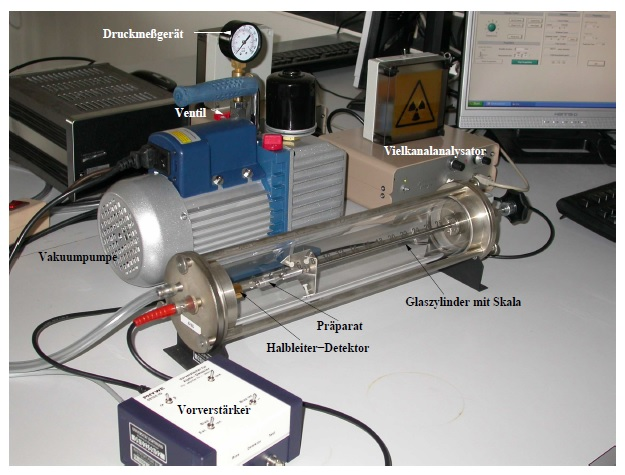
\includegraphics[width=0.8\linewidth]{Aufbau.jpg}
	\caption{Aufbau zur Bestimmung der Reichweite.\cite[3]{anleitung701}}
	\label{fig:aufbau}
\end{figure}

\subsection{Bestimmung der Reichweite}
Nach Einstellen der Diskreminatorschwelle wird das Präparat so nah an den Detektor herangeführt, dass dieser gerade wieder anfängt, $\alpha$-Teilchen zu registrieren. Anschließend wird das Präparat fixiert und der Glaskolben 
evakuiert. Nun wird einmal für die Länge $l$\,=\,1,5\,cm  und $l$\,=\,2\,cm in $\SI{50}{\milli\bar}$-Schritten die Energieverteilung gemessen und über jeweils $\SI{120}{\second}$ Messungen durchgeführt. Zu jedem Druck 
wird nun der Kanal des Energiemaximums und die Gesamtpulszahl notiert. Es wird von einer linearen Energieskala ausgegangen und so kann die Energie der $\alpha$-Teilchen in Abhängigkeit vom Druck bestimmt werden. Bei 
$\SI{0}{\milli\bar}$ entspricht dies etwa einem Kanal von $\SI{4}{\mega\electronvolt}$.

\subsection{Statistik des radioaktiven Zerfalls}
Anschließend soll die Statistik des radioaktiven Zerfalls überprüft werden, indem bei vollkommen evakuiertem Zylinder $100$ Messungen zu je $\SI{10}{\second}$ durchgeführt in denen die Anzahl der Zerfälle aufgenommen wird. 
Danach werden hieraus die Varianz und der Mittelwert errechnet und mit einer Gauß- und Poissonverteilung verglichen. 